\PID Нацртати континуалне сигнале:
(а) јединични правоугаони импулс, $\rect(t)$, 
(б) јединични троугаони импулс, $\operatorname{tri}(t)$, 
(в) функцију $\sinc(t)$; и дискретне сигнале 
(г) дискретан јединични импулс, $\updelta[n]$, 
(д) дискретнан јединични низ, $\uu(t)$, и 
(ђ) дискретну праовоугаону функцију полуширине 2, $\rect_2(t)$.
\\[2mm]

\textsc{\underline{Решење}}:
\begin{figure}[ht!]
    \hspace*{0pt}\hfill
    \begin{subfigure}[c]{0.33\textwidth}
        \centering
        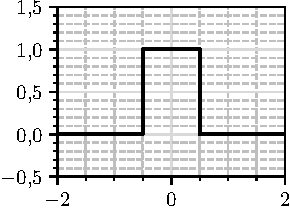
\includegraphics[scale=1]{fig/rect_plot.pdf}
        \caption{$\rect(t)$}
    \end{subfigure}
    \hspace*{0pt}\hfill
    \begin{subfigure}[c]{0.3\textwidth}
        \centering
        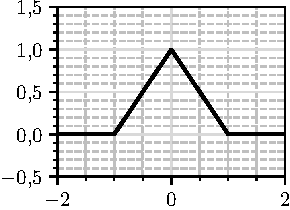
\includegraphics[scale=1]{fig/tri_plot.pdf}
        \caption{$\operatorname{tri}(t)$}
    \end{subfigure}
    \hfill
    \hspace*{0pt}
    \hspace*{0pt}\hfill
    \begin{subfigure}[c]{0.3\textwidth}
        \centering
        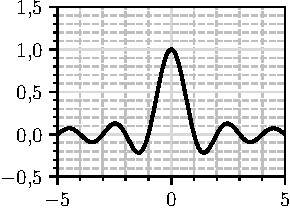
\includegraphics[scale=1]{fig/sinc_plot.pdf}
        \caption{$\sinc(t)$}
    \end{subfigure}
    \hspace*{0pt}\hfill
    \begin{subfigure}[c]{0.3\textwidth}
        \centering
        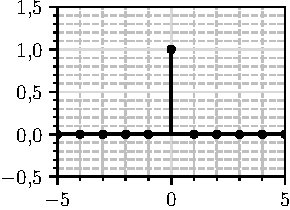
\includegraphics[scale=1]{fig/delta_dt_plot.pdf}
        \caption{$\updelta[n]$}
    \end{subfigure}
    \hfill
    \begin{subfigure}[c]{0.3\textwidth}
        \centering
        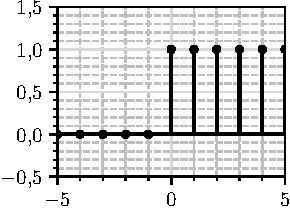
\includegraphics[scale=1]{fig/u_dt_plot.pdf}
        \caption{$\uu[n]$}
    \end{subfigure}
    \hfill
    \begin{subfigure}[c]{0.3\textwidth}
        \centering
        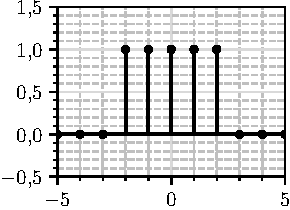
\includegraphics[scale=1]{fig/rect_dt_plot.pdf}
        \caption{$\rect_2[n]$}
    \end{subfigure}
    \hfill
    \hspace*{0pt}
    \caption{}
\end{figure}
\vspace*{-10mm}